\begin{itemize}
\item Conceptos básicos 
    \begin{enumerate}
    \item ¿ La {\it "propiedad"} es una propiedad intensiva o extensiva? Analizar la pregunta para las siguientes {\it propiedades}:\\
    Volumen, masa, densidad, viscosidad, temperatura, compresibilidad, peso, deformación.
    \item ¿ La {\it "magnitud"} es una magnitud escalar, vectorial o tensorial? Analizar la pregunta para las siguientes {\it magnitudes}:\\
    Velocidad, aceleración, temperatura, esfuerzo viscoso, estado de deformación, presión.
    \item ¿ Qué tipo de sistema es un volumen de control? ¿Qué utilidad tiene en mecánica de los fluidos?
    \item ¿ En qué consiste un modelo? Dibujar un esquema donde se muestre la relación entre
    el problema físico, el problema matemático derivado y la solución obtenida.
    \item Nombrar posibles características que pueden describir un modelo de {\bf flujo}. Por otro lado, contrastarlas con las
    posibles propiedades de un {\bf fluido}.
    \item ¿Cuál es la característica principal de un flujo estacionario?
    \end{enumerate}
    
  \item Estática
    \begin{enumerate}
    \item Escribir la formulación vectorial del principio general de la hidrostática:
    \item Definición general de fuerza hidrostática sobre una superficie:
    \item Definición general de torque respecto del punto $0$ provocado por fuerza hidrostática sobre una superficie:
    \item Definir cuáles de las siguientes afirmaciones son correctas para la figura adjunta \ref{fig:hidrostat}.

      \begin{figure}[!ht]
      \centering
      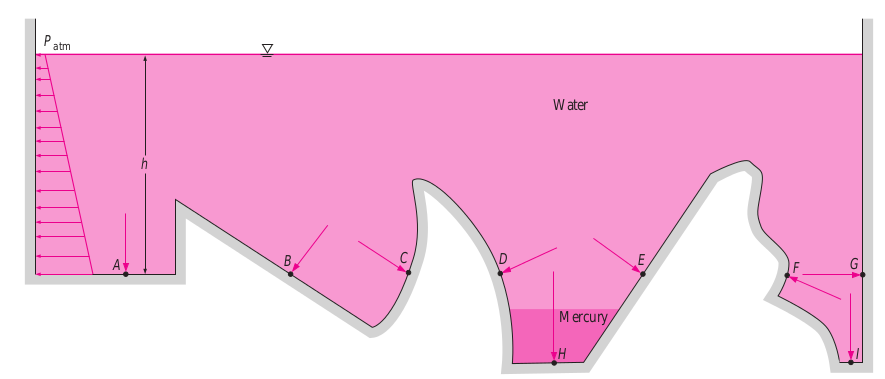
\includegraphics[width=15cm]{hidrostat.png}
      \caption{Caso hidrostática}
      \label{fig:hidrostat}
      \end{figure}

      \begin{itemize}
      \item $p_A = p_B= p_C= p_D= p_F$ \_\_\_\_
      \item $p_A = p_I$ \_\_\_\_
      \item $p_H = p_I$ \_\_\_\_
      \item $p_A = p_{atm}+\rho g h$ \_\_\_\_
      \item $\overline{F}_A = \overline{F}_B= \overline{F}_C= \overline{F}_D= \overline{F}_F$ \_\_\_\_
      \end{itemize}
      
      %   
    \item La fuerza de empuje sobre un cubo sumergido en agua sólo hasta la mitad de su altura es:

    $F_{empuje} =$ 


    \end{enumerate}
    
    \clearpage
    
   \item Cinemática
    \begin{enumerate}
    \item Dado un {\bf flujo incompresible}, escribir la ecuación de continuidad en su forma vectorial: 
    \item Escribir la derivada material desde el punto de vista Lagrangiano, Euleriano:\\
    \vskip 1.cm
    
    \item Escribir la ecuación de Bernoulli. Indicar con una cruz cuáles de las siguientes son hipótesis
    necesarias para la aplicación de dicha ecuación.

    \vskip 1.cm

      \begin{itemize}
      \item Flujo incompresible. \_\_\_\_
      \item Flujo ideal. \_\_\_\_
      \item Flujo estacionario. \_\_\_\_
      \item La única fuerza de cuerpo sobre el fluido es el peso. \_\_\_\_
      \end{itemize}

    \end{enumerate}
    
   \item Dinámica
    \begin{enumerate}
        \item Escriba la fórmula de cálculo para el número de Reynolds. $Re = $

    \end{enumerate}
    
   \item Flujos confinados
    \begin{enumerate}
    \item Escribir la fórmula de Darcy ($f$) para el cálculo de la pérdida de carga en una cañería.¿En qué unidad se obtiene el resultado?

    \vskip 1.cm

    \end{enumerate}
    
   \item Flujos compresibles
    \begin{enumerate}
    \item Escriba la fórmula de cálculo para el número de Mach. $Ma = $
    \item La velocidad de propagación del sonido ($c$) en un fluido depende de la velocidad media de flujo ($u$).
      \begin{itemize}
      \item Verdadero. \_\_\_\_
      \item Falso. \_\_\_\_
      \end{itemize}


    \end{enumerate}
    
   \item Fundamentos de máquinas hidráulicas
    \begin{enumerate}
    \item ¿Cómo se comporta la densidad de un fluido dentro de una máquina hidráulica?
    \end{enumerate}
    
   \item Bombas centrífugas
    \begin{enumerate}
    \item ¿Cuál es la principal función de una bomba hidráulica?

    \vskip 1.cm


    \end{enumerate}
    
   \item Turbinas hidráulicas
    \begin{enumerate}
    \item ¿Cuál es la principal función de una turbina hidráulica?
    \item Una turbina con número específico de revoluciones elevado es más eficiente:
		\begin{itemize}
			\item A caudales altos \_\_\_
   			\item A caudales bajos \_\_\_
		\end{itemize}    
    \end{enumerate}

    \vskip 1.cm
\end{itemize}